In diesem Kapitel beschreiben wir zunächst, welche grundlegenden Arbeitsprozesse
wir verwendet haben. Anschließend schildern wir den zeitlichen Ablauf des
Projektes.

\subsection{Grundlegende Arbeitsweise und -aufteilung}
Die gesamte anstehende Arbeit wurde in mehrere Unteraufgaben aufgeteilt, die wir
zumeist einzeln erledigten.
In besonderen Fällen wichen wir jedoch auf Pair Programming aus. Wir trafen uns
regelmäßig einmal die Woche, um unseren Fortschritt festzustellen und gemeinsam
am Projekt weiterzuarbeiten. In einer einfachen Textdatei wurden Milestones
definiert und festgelegt, bis wann von wem welche Funktion implementiert sein
sollte (vgl. Bild~\ref{figure:assignee}).

\begin{figure}[htbp]
  \centering

    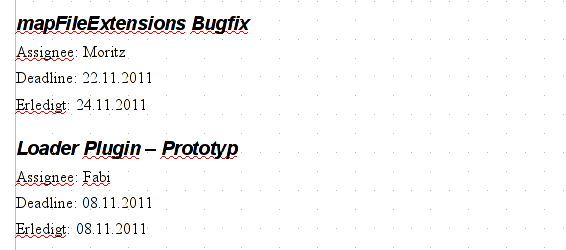
\includegraphics[width=0.7\textwidth]{gfx/assignee.png}

  \caption{Ausschnitt unserer Roadmap.}
  \label{figure:assignee}
\end{figure}

Zu Beginn des Projektes haben wir zunächst mit den UH-Entwicklern gesprochen,
um festzustellen, welche Anforderungen der Editor erfüllen sollte. Hierzu
haben wir uns informell mit einigen der Entwicklern im IRC unterhalten und
festgestellt, dass der bestehende FIFE-Editor eine gute Basis für den Map
Editor darstellt.

Anschließend haben wir uns in den bestehenden Code des Editors und den
Ladeprozess von UH eingelesen, um herauszufinden, welche Schwierigkeiten bei der
Implementierung bestehen könnten und wie eine funktionstüchtige Architektur
aussehen könnte.
In einer kurzen Diskussion im FIFE IRC-Channel haben wir herausgefunden, dass
derzeit am FIFE-Editor gearbeitet wird, um die Integration von anderen
Kartenformaten zu ermöglichen, dass dieser Prozess jedoch noch nicht
abgeschlossen ist. Nach gründlicher Überlegung haben wir damit begonnen,
grundsätzliche Probleme zu identifizieren, bevor wir mit der eigentlichen Arbeit
-- dem Implementieren der Loader und Saver Plugins -- beginnen konnten. Die sich
abzeichnenden Aufgaben strukturierten wir und hielten sie in einer Roadmap fest
(siehe Bild~\ref{figure:assigneeq}).

\subsection{Zeitlicher Ablauf des Projekts}
 Es stellte sich heraus, dass
prinzipiell mit dem Loader-Plugin direkt begonnen werden konnte, das MapSaver
Plugin jedoch einige Vorarbeit an FIFE selbst erforderte. Grundsätzlich fuhren
wir ab da die Entwicklung des MapLoaders und MapSavers Plugin weitgehend
parallel zueinander. Hierzu teilten wir die Arbeit auf, da sich abzeichnete,
dass beides ungefähr gleichen Arbeitsaufwand bedeutete.

Während unserer Arbeit an den Plugins stellten sich einige Unzulänglichkeiten
des FIFE Editors heraus. Um diese zu beheben, schrieben wir etliche Patches für
FIFE, die z.B.
Bugs im Dateiauswahldialog des Editors behoben. Für das Saver-Plugin fehlte die
Infrastruktur-Unterstützung durch FIFE komplett und musste eigens erstellt
werden. Die resultierenden Patches haben wir anschließend in den FIFE Bugtracker
gestellt, von wo sie von einem der FIFE Entwickler gemerged wurden.


Um Laden UH Objekte zu laden, war eine weitere intensive Beschäftigung mit dem
FIFE Editor Code und dem UH Kartenformat nötig. Solbald die Objekte im Editor
geladen werden konnten, präsentierten wir unseren Fortschritt in einem der
wöchentlichen Meetings von UH.

Da zu dieser Zeit gerade größere Umbauarbeiten an der Architektur des Spiels vorgenommen wurden,
kam es zu einem Konflikt mit unserem Editor-Code. Änderungen am Spiel zwangen uns, einen Teil
des Codes neu zu schreiben, um mit den neuen Features des Spiels kompatibel zu bleiben. Dies
hätte allerdings nicht vermieden werden können, da die Änderungen bereits vor dem Beginn des
Editor-Projekts geplant waren und nicht verschoben werden konnten. Da wir bereits frühzeitig
auf einem weiter fortgeschrittenen Branch des Git-Repositories gearbeitet hatten, war der
Umfang der nötigen Änderungen noch angemessen.


Parallel trieben wir die Entwicklung des MapSavers voran. Wir begannen damit,
zunächst nur Buildings abzuspeichern, da dies wesentlich einfacher war, als
Groundtiles. Die resultierenden Karten zeigten im Nichts hängende Gebäude, was
jedoch schon ein großer Fortschritt war.
Anschließend kümmerten wir uns um das Abspeichern der Groundtiles. Dies
erforderte das Erstellen eines Partitionierungsalgorithmus, der zusammengehörige
Tiles automatisch erkennt und zu einer Insel gehörig abspeichert.

Ein großer Punkt war jedoch zu diesem Zeitpunkt noch offen: Die Rotation von
Objekten auf der Karte.
Bisher lud der MapLoader die Objekte noch ohne Rotation, sie zeigten folglich
alle in die gleiche Richtung. Auch der MapSaver speicherte keine Rotationsdaten.
Nach einiger Recherche und ein paar erfolglosen Versuchen, die Rotation der
Gebäude richtig zu setzen, wandten wir uns an die UH-Entwickler.
Wie sich herausstellte war der Code-Abschnitt, der im Spiel die Gebäude rotiert
relativ alt und niemand konnte sich mehr erinnern, wie er funktioniert
(Original-Kommentar ``nobody actually knows how the code below works.'').
Es gab auch keine Dokumentation zu diesem Punkt. Leider stolperten wir sehr oft
über genau diesen Code.

Daraufhin entschlossen wir uns, das Problem in einer Pair-Programming-Sitzung anzugehen. Dies hatte
den Vorteil, dass wir das Problem gleichzeitig und mit zwei unterschiedlichen Sichtweisen betrachten
konnten, während wir zusammen aktiv an einer Lösung arbeiteten. Hierdurch gelang es uns, eine funktionierende
Rotation der Objekte im MapLoader zu implementieren.

Über die Weihnachtszeit erfolgte dann ein weiterer großer Umbau der Architektur
von UH. Das gesamte Design aller auf der Karte platzierten Objekte wurde
umgestellt, woraufhin unser Edior-Code zunächst nicht mehr funktionstüchtig war.
Nach einem vollen Tag an Arbeit waren die Plugins jedoch wieder einsatzfähig.


Schlussendlich wurde durch ein FIFE-Update das Rückgeben von Koordinatenwerten
im Editor ungenau: Statt $[45^\circ, 135^\circ, 225^\circ, 315^\circ]$ wurden
nun Werte wie $44^\circ, 46^\circ$ etc. von der {\tt getRotation()}-Methode des
Editors zurückgegeben. Da UH grundsätzlich gegen den FIFE trunk kompiliert wird,
mussten wir hierfür zusätzlich eine Korrekturfunktion schreiben. Allein das
Debugging nahm Stunden in Anspruch.

